\documentclass[a4paper, 12pt]{article}
\usepackage[UTF8]{ctex}
\usepackage{float}
\usepackage{graphicx}

\begin{document}
	\title{系统开发工具基础实验报告(一)}
	\author{22110032031 张希敏}
	\date{\today}
	\maketitle
	
	\pagenumbering{roman}
	\tableofcontents
	\newpage
	\pagenumbering{arabic}
	
	\section{练习主题}
	\paragraph{(1)版本控制(Git)}
	
	\paragraph{(2)Latex 文档编辑}
	
	\section{练习内容}
	
	\subsection{四个题目}
	
	\subsubsection{题目一}
	克隆课程网站的仓库。
	
	\paragraph{答:}
	使用git clone命令,如图:
	
	\begin{figure}[h]
		\centering
		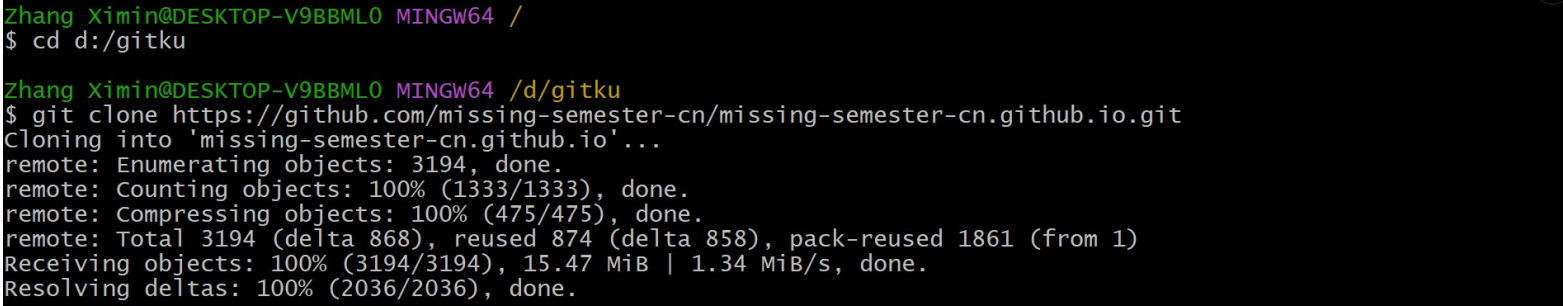
\includegraphics[width=1\textwidth]{001.jpg}
	\end{figure}
	
	\paragraph{(1)将版本历史可视化并进行探索。}
	
	\paragraph{答:}
	输入git log --all --graph --decorate查看结果。
	
	\begin{figure}[H]
		\centering
		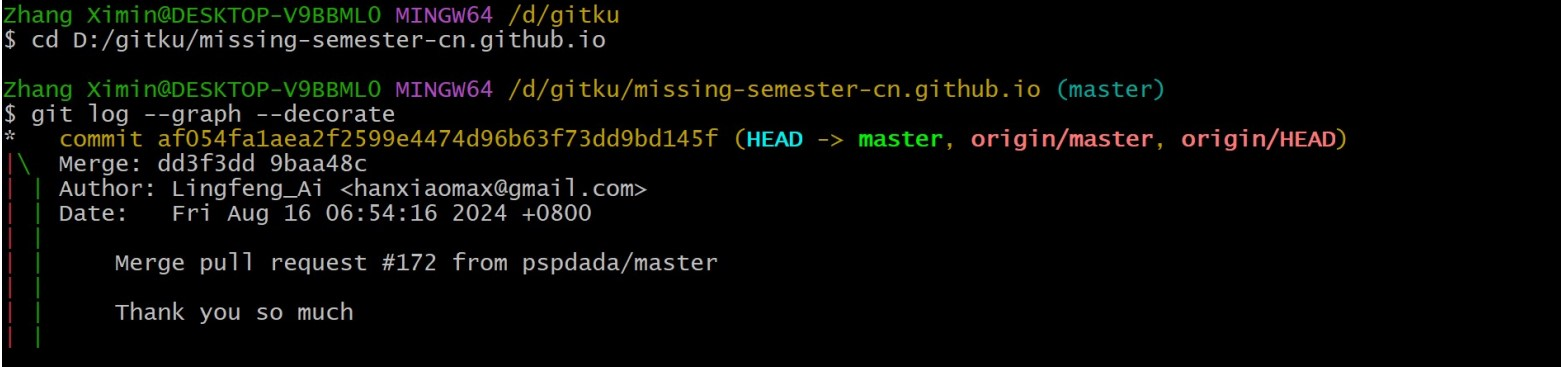
\includegraphics[width=1\textwidth]{002.jpg}
		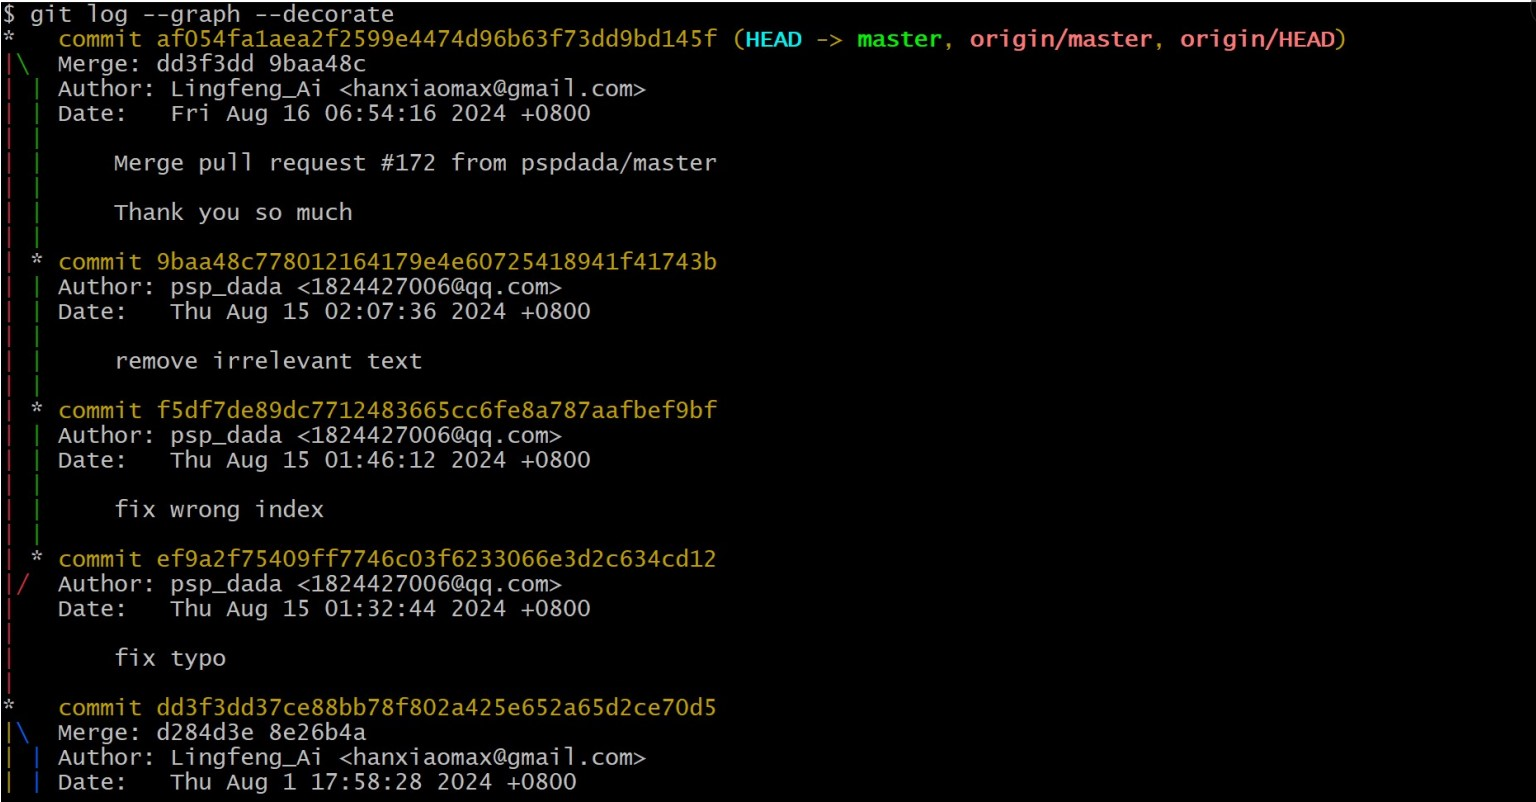
\includegraphics[width=1\textwidth]{003.jpg}
	\end{figure}
	
	\paragraph{(2)是谁最后修改了 README.md 文件?}
	
	\paragraph{答:}
	输入git log -1 README.md查看结果,如图:
	
	\begin{figure}[H]
	\centering
	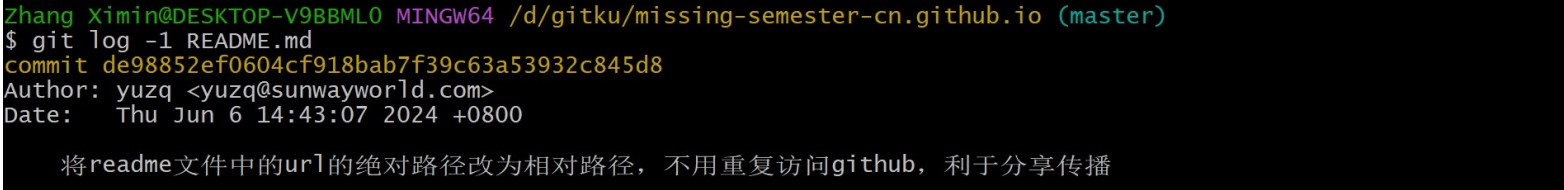
\includegraphics[width=1\textwidth]{004.jpg}
	\end{figure}

	\paragraph{(3)最后一次修改 \_config.yml 文件中 collections: 行时的提交信息是什么?}
	
	\paragraph{答:}
	输入 git blame \_config.yml | grep collections
	
	git show --pretty=format:"\%s" a88b4eac
	
	结果如图:
	
	\begin{figure}[H]
		\centering
		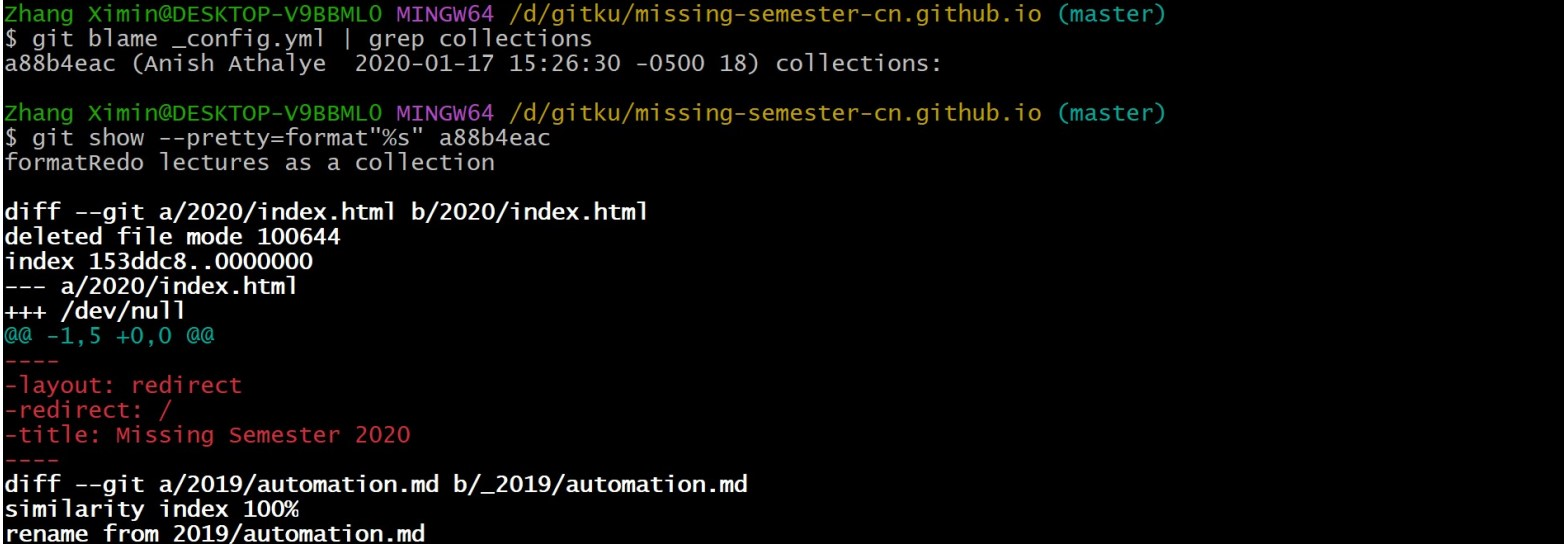
\includegraphics[width=1\textwidth]{005.jpg}
	\end{figure}
	
	\subsubsection{题目二}
	向仓库中添加一个文件并添加提交信息,然后将其从历史中删除。
	
	\paragraph{答:}
	提交敏感信息文件:
	
	echo "password123">my\_password
	
	git add .
	
	git commit -m "add password123 to file"
	
	git log HEAD
	
	清除提交记录:
	
	git filter-branch --force --index-filter\
	
	'git rm --cached --ignore-unmatch ./my\_password' \
	
	--prune-empty --tag-name-filter cat -- --all
	
	检查文件是否删除,如图:
	
	\begin{figure}[H]
		\centering
		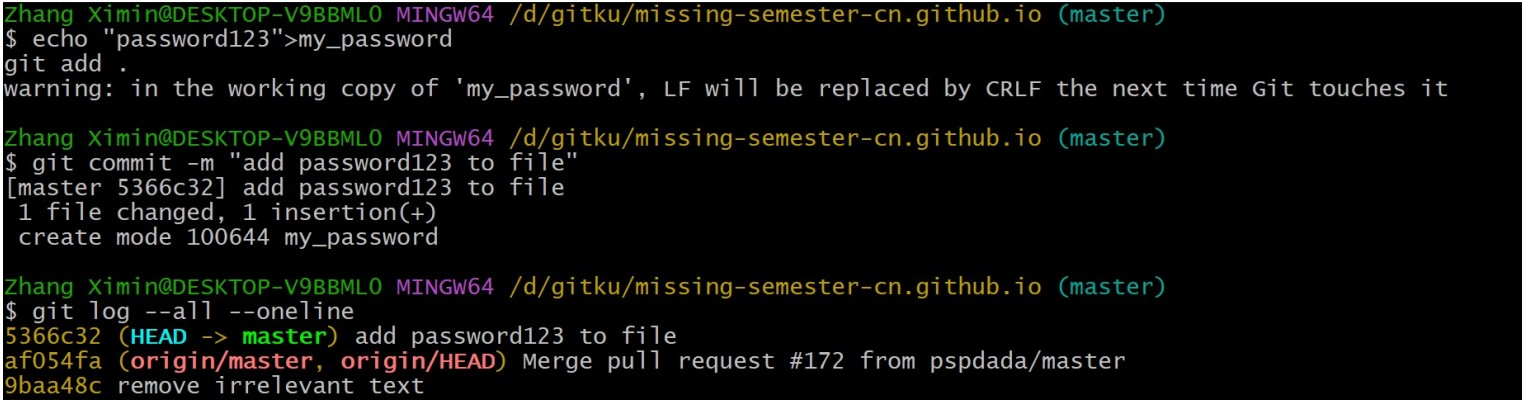
\includegraphics[width=1\textwidth]{006.jpg}
		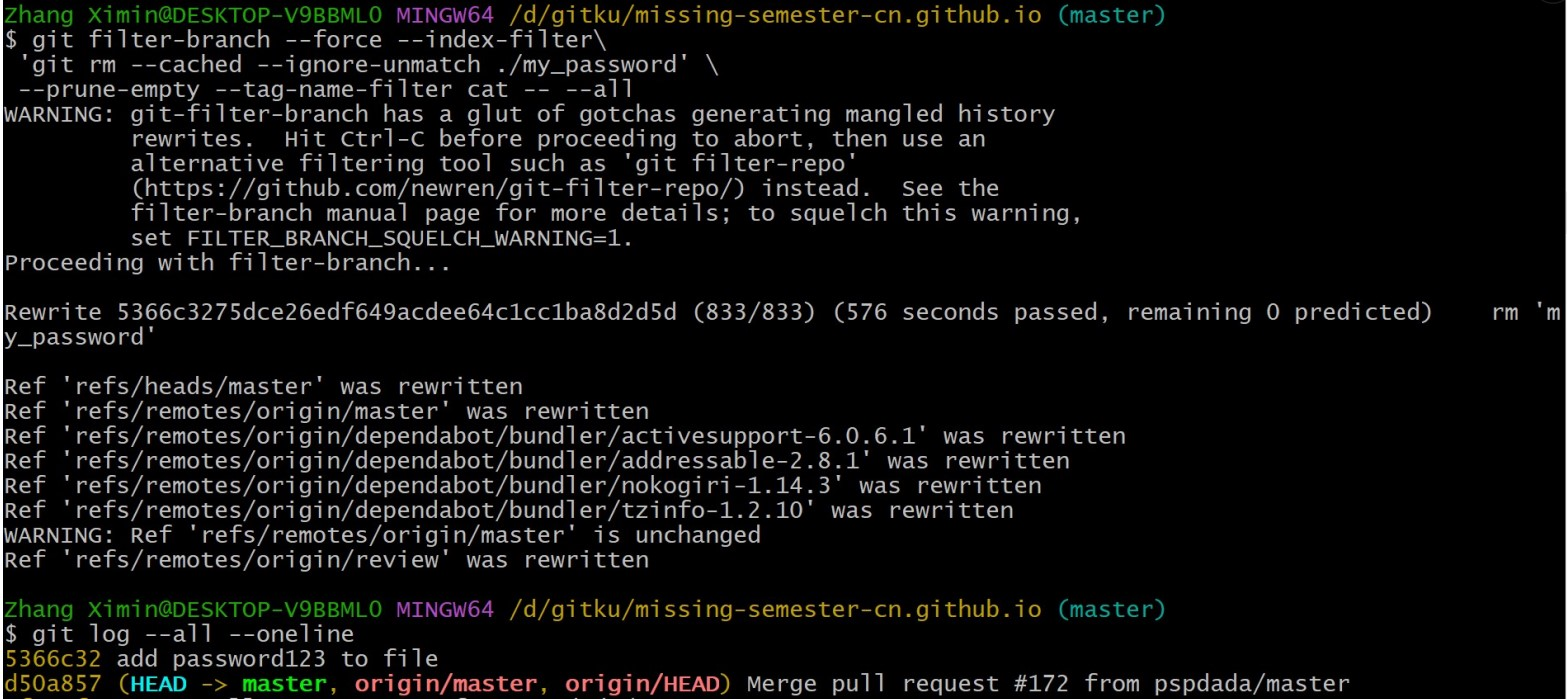
\includegraphics[width=1\textwidth]{007.jpg}
		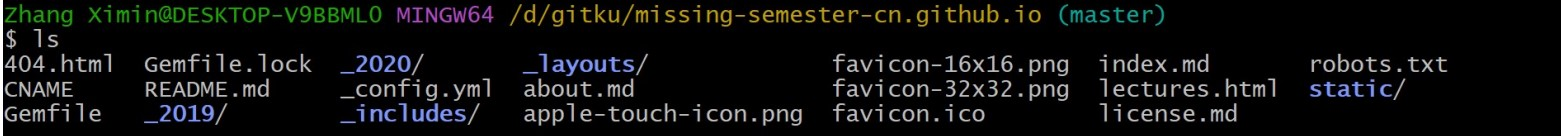
\includegraphics[width=1\textwidth]{008.jpg}
	\end{figure}
	
	\subsubsection{题目三}
	从 GitHub 上克隆某个仓库,修改一些文件。当您使用 git stash 会发生什么?当您执行 git log --all --oneline 时会显示什么?通过 git stash pop 命令来撤销 git stash 操作,什么时候会用到这一技巧?
	
	\paragraph{答:}
	
	使用 git stash 会将当前工作目录中的所有修改保存到一个新的“stash”中,并将工作目录和暂存区恢复到最近一次提交的状态。这使得修改被安全保存的同时,工作目录是干净的,没有未提交的修改。
	
	执行 git log --all --oneline 命令会显示所有分支的提交历史,每个提交显示一行。
	
	git stash pop 命令用于将最近一次stash的修改重新应用到当前的工作目录和暂存区中,使用场景有需要在不同的任务中切换的情景,或者已经完成了其他任务要回到之前stash的修改点继续工作的情景等。
	
	\begin{figure}[H]
		\centering
		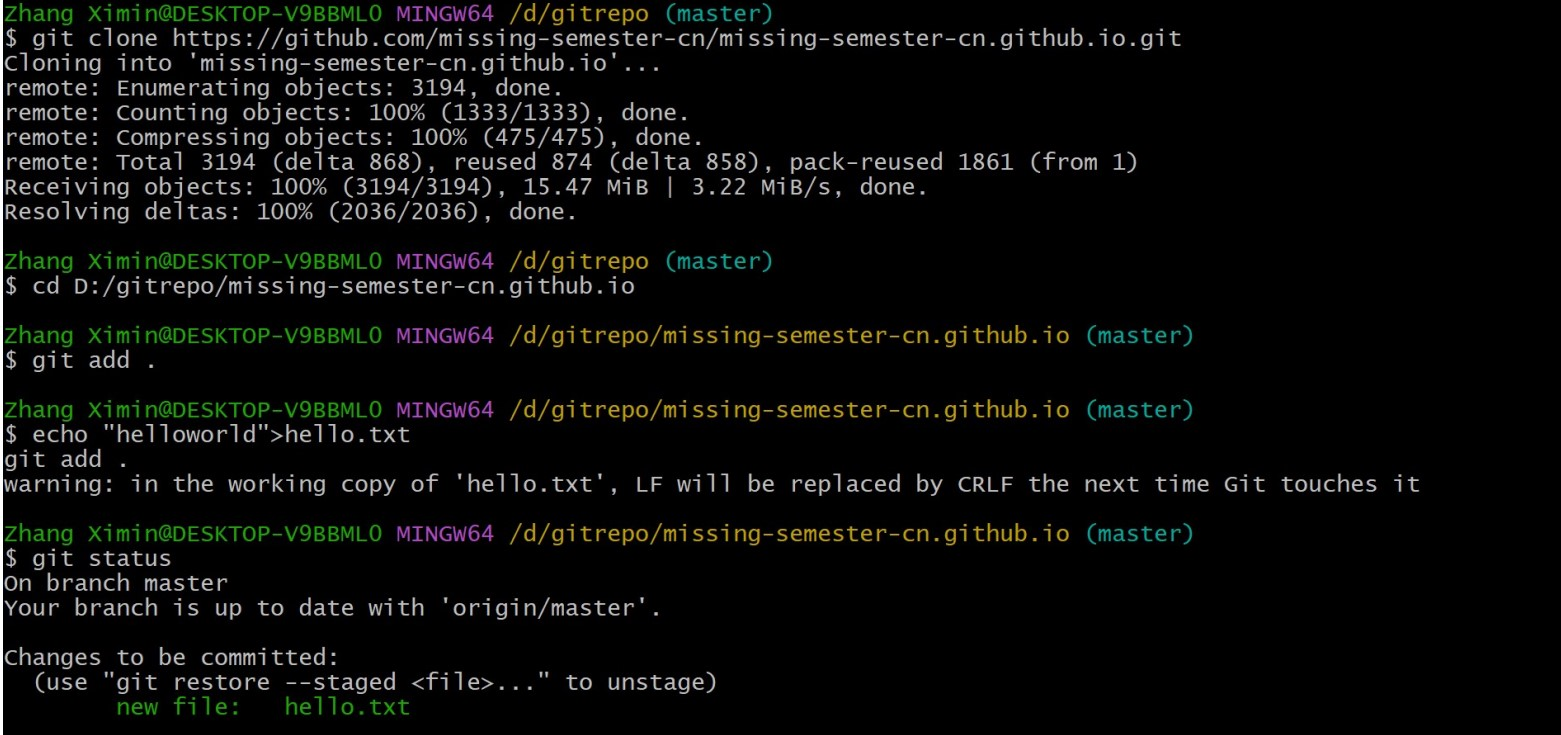
\includegraphics[width=1\textwidth]{009.jpg}
		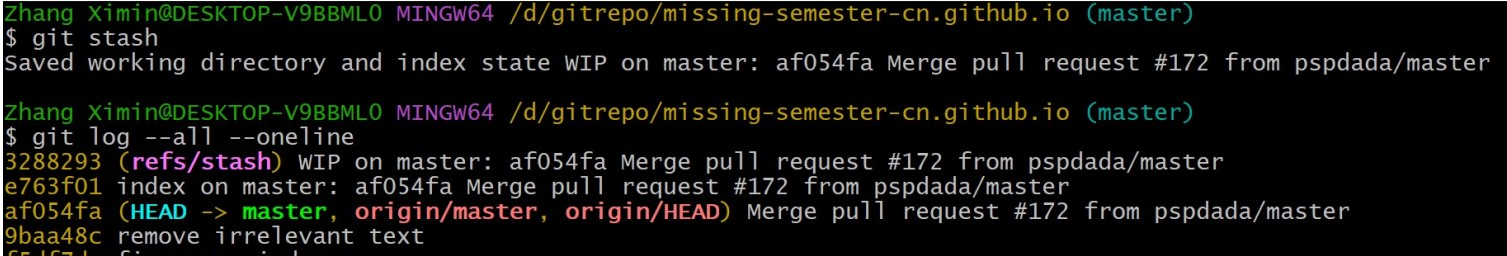
\includegraphics[width=1\textwidth]{010.jpg}
		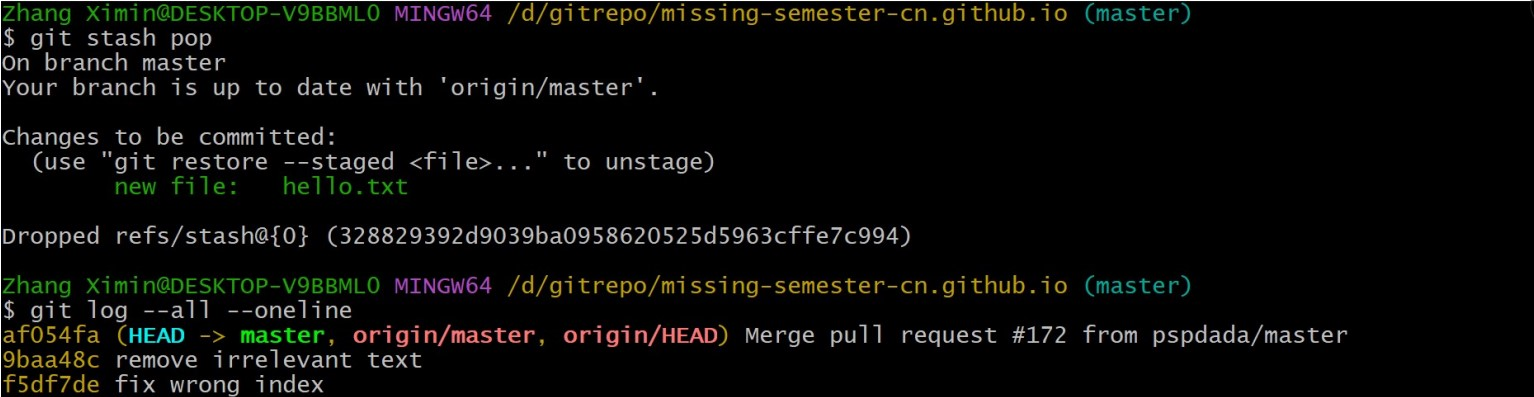
\includegraphics[width=1\textwidth]{011.jpg}
	\end{figure}
	
	\subsubsection{题目四}
	请在 ~/.gitconfig 中创建一个别名,使您在运行 git graph 时,您可以得到 git log --all --graph --decorate --oneline 的输出结果。
	
	\paragraph{答:}
	修改本地环境中的gitconfig文件,在最后添加别名[alias]:

		graph = log --all --graph --decorate --oneline
		
	结果如图:
	
	\begin{figure}[H]
		\centering
		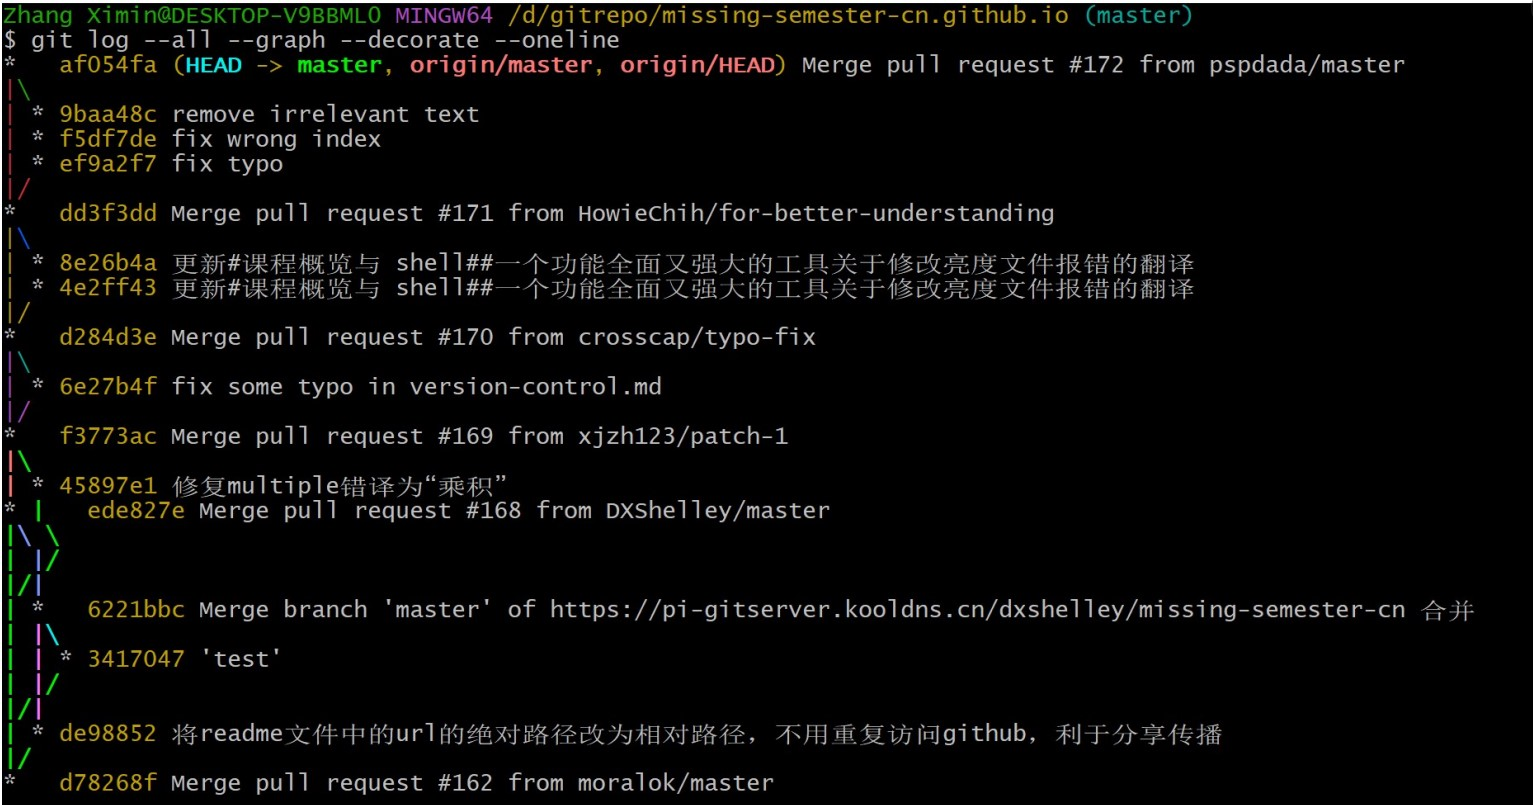
\includegraphics[width=1\textwidth]{012.jpg}
		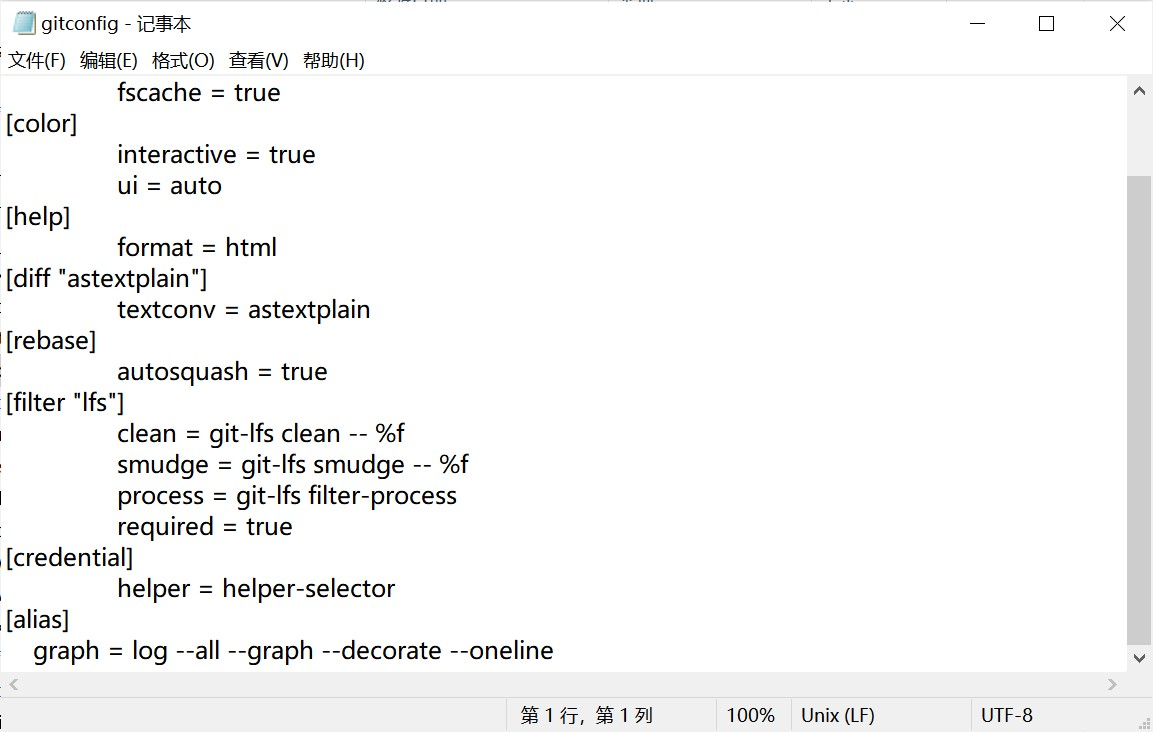
\includegraphics[width=1\textwidth]{013.jpg}
		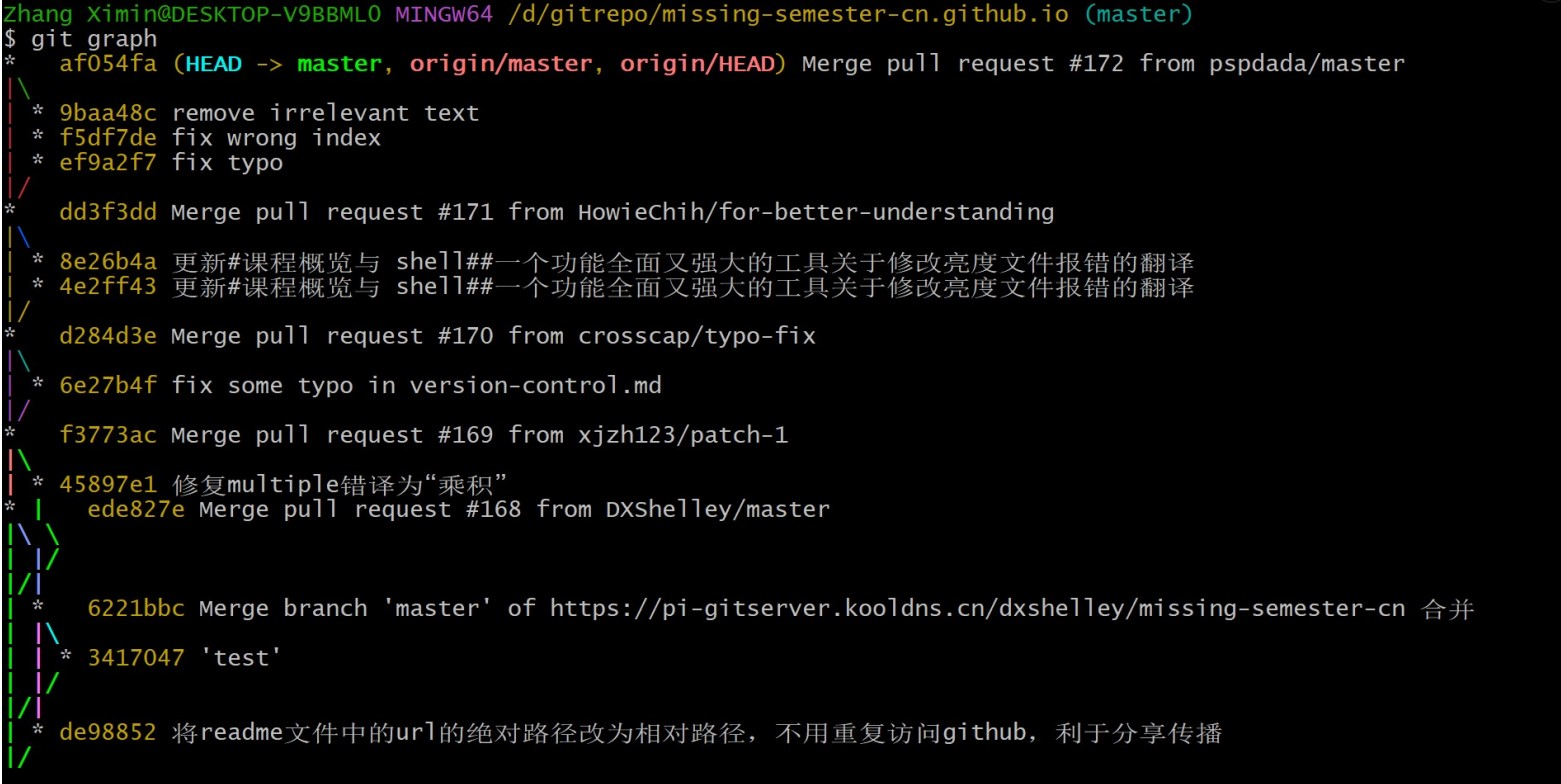
\includegraphics[width=1\textwidth]{014.jpg}
	\end{figure}
	
	\subsection{20个实例}
	
	\paragraph{(1)git init:}
	创建一个新的 git 仓库,其数据会存放在一个名为 .git 的目录下。
	
	\begin{figure}[H]
		\centering
		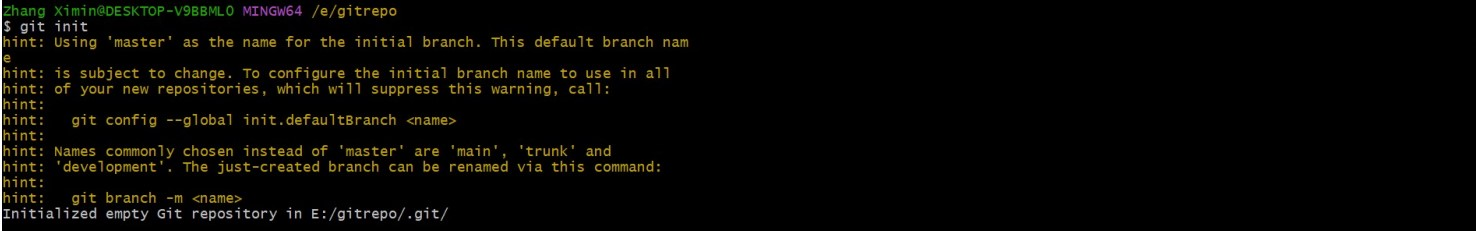
\includegraphics[width=1\textwidth]{015.jpg}
	\end{figure}
		
	\paragraph{(2)git add <filename>:}	
	添加文件到暂存区。
	
	\begin{figure}[H]
		\centering
		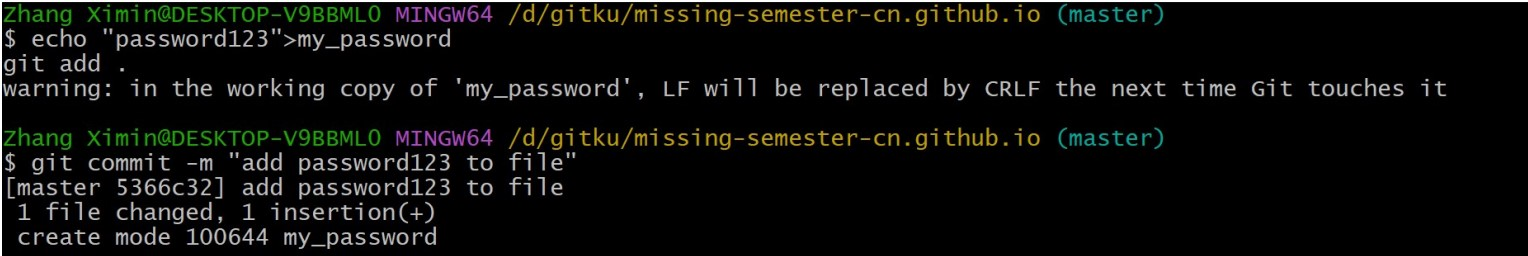
\includegraphics[width=1\textwidth]{017.jpg}
	\end{figure}	
		
	\paragraph{(3)git status:}	
	显示当前的仓库状态。
	
	\begin{figure}[H]
		\centering
		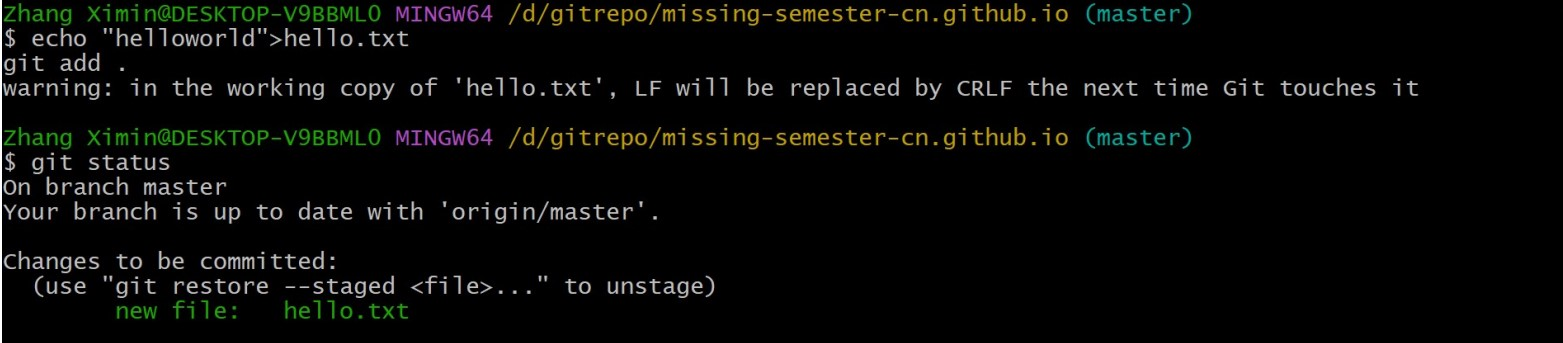
\includegraphics[width=1\textwidth]{016.jpg}
	\end{figure}
	
	\paragraph{(4)git commit:}	
	创建一个新的提交。
	
	\begin{figure}[H]
		\centering
		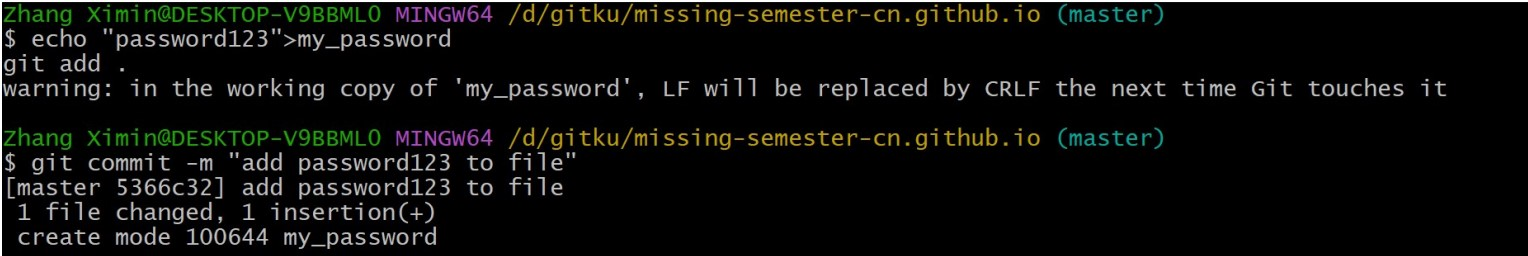
\includegraphics[width=1\textwidth]{017.jpg}
	\end{figure}
	
	
	\paragraph{(5)git log:}
	显示历史日志。
	
	git log --all --graph --decorate: 可视化历史记录	
	
	\begin{figure}[H]
	\centering
	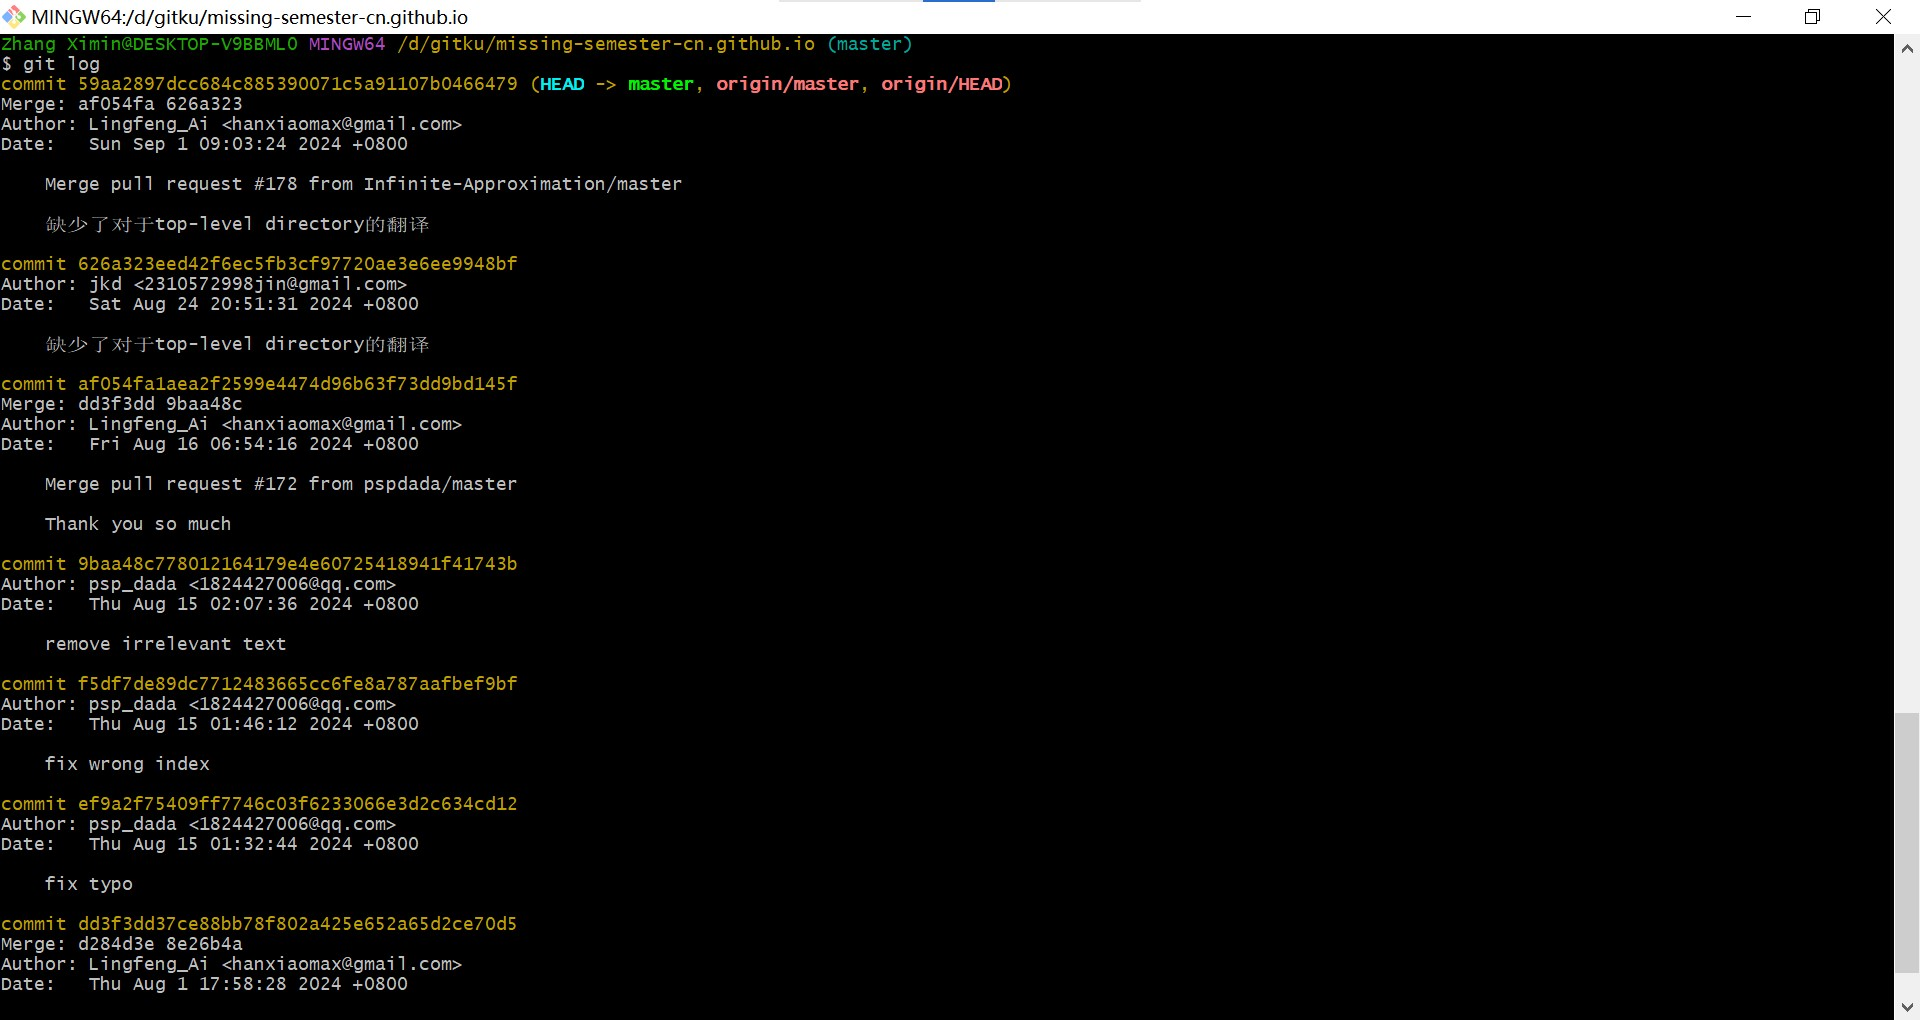
\includegraphics[width=1\textwidth]{018.jpg}
	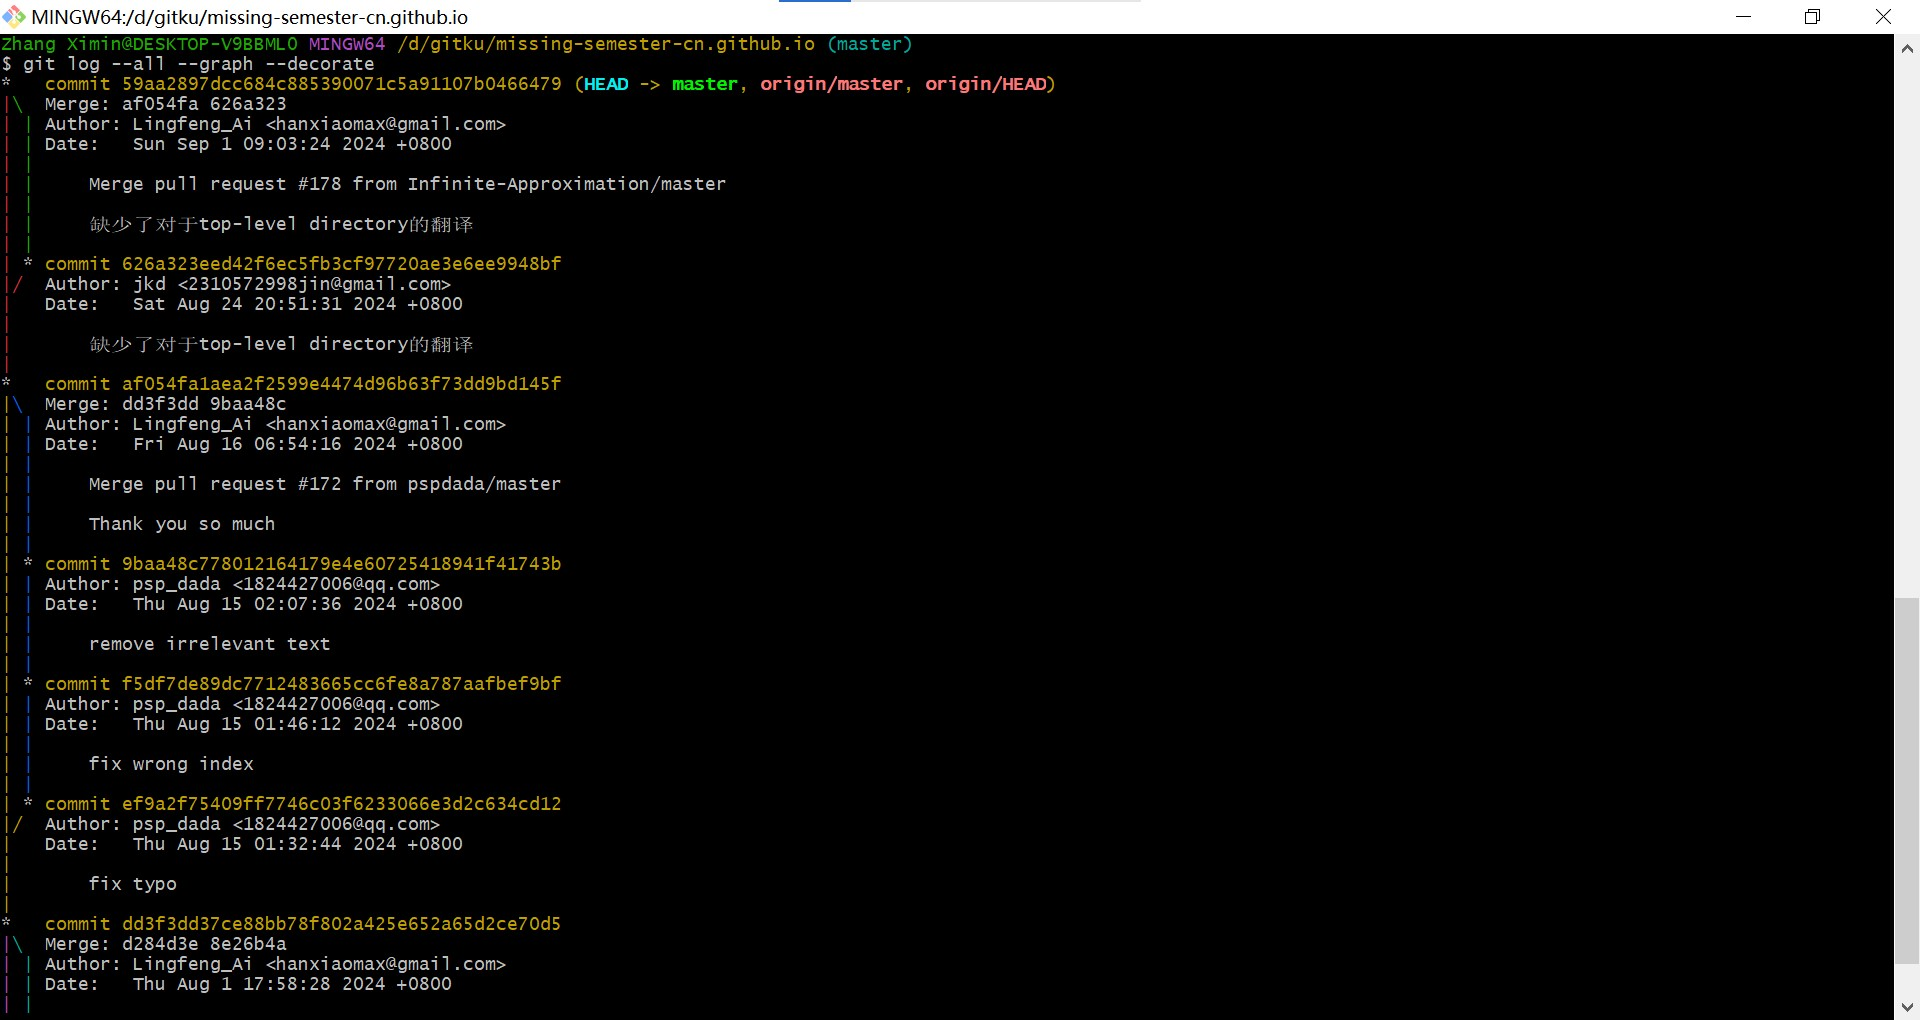
\includegraphics[width=1\textwidth]{019.jpg}
	\end{figure}
	
	\paragraph{(6)git help <command>:}	
	获取 git 命令的帮助信息。
	
	\begin{figure}[H]
		\centering
		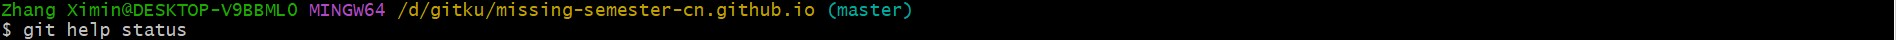
\includegraphics[width=1\textwidth]{020.jpg}
		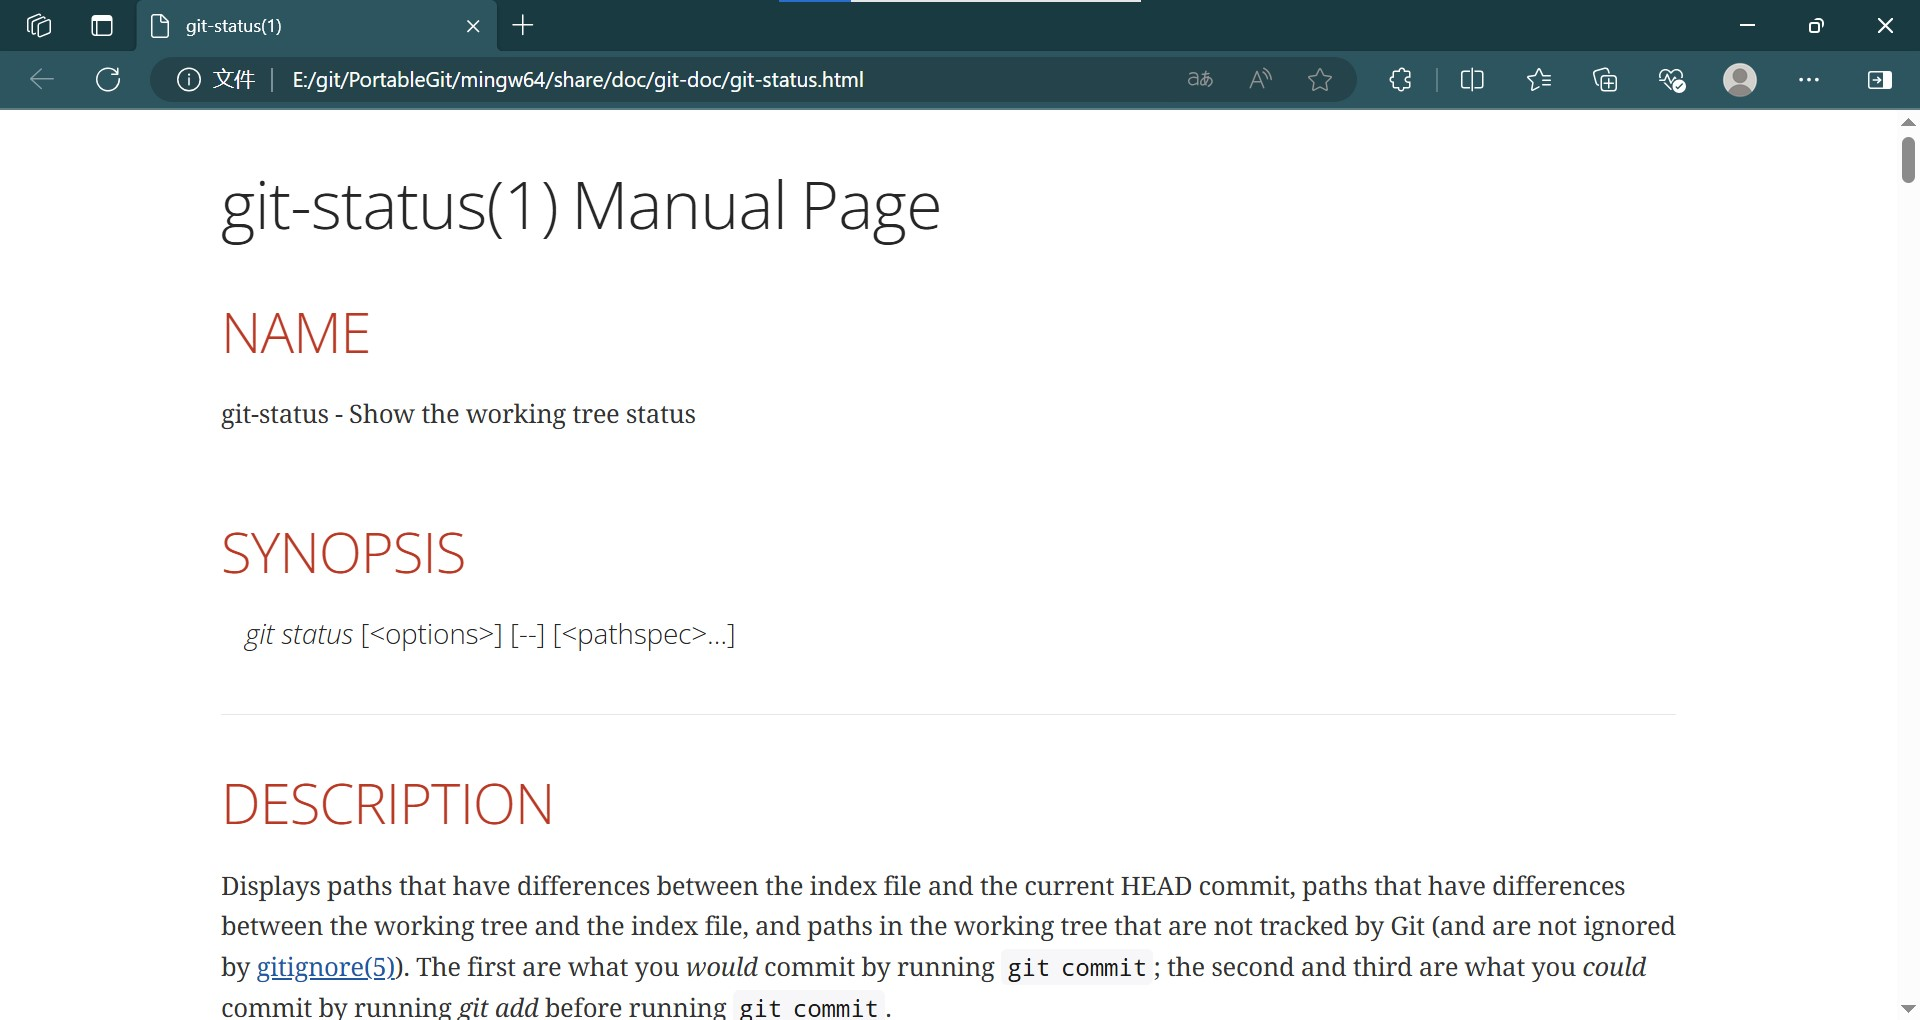
\includegraphics[width=1\textwidth]{021.jpg}
	\end{figure}
	
	\paragraph{(7)git checkout <revision>:}
	更新 HEAD 和目前的分支。	
	
	\begin{figure}[H]
		\centering
		
\includegraphics[width=1\textwidth]{022.jpg}
	\end{figure}
	
	\paragraph{(8)git branch:}	
	显示分支。
	
	git branch <name>: 创建分支。
	
	git branch -d <name>:删除分支。
	
	\begin{figure}[H]
		\centering
		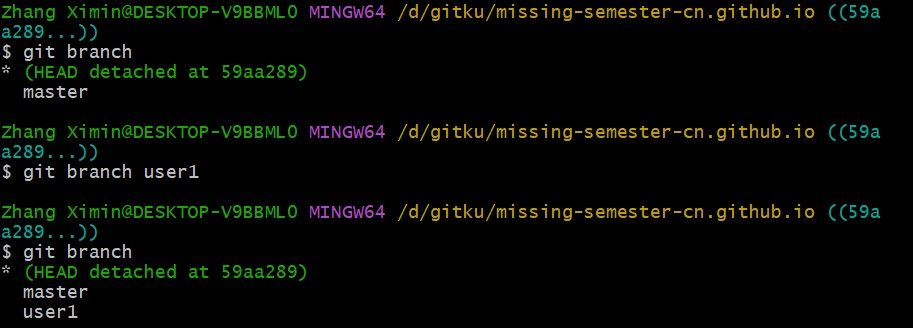
\includegraphics[width=1\textwidth]{023.jpg}
		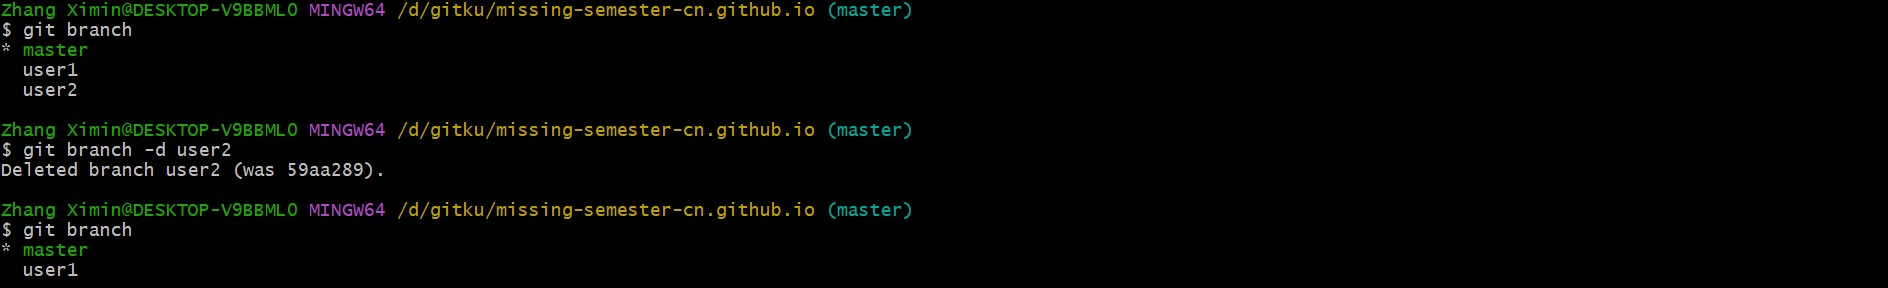
\includegraphics[width=1\textwidth]{026.jpg}
	\end{figure}
	
	\paragraph{(9)git checkout -b <name> 或者 git switch -c <name>:}	
	创建分支并切换到该分支。
	
	git checkout <name> 或者 git switch <name>:切换分支。
	
	\begin{figure}[H]
		\centering
		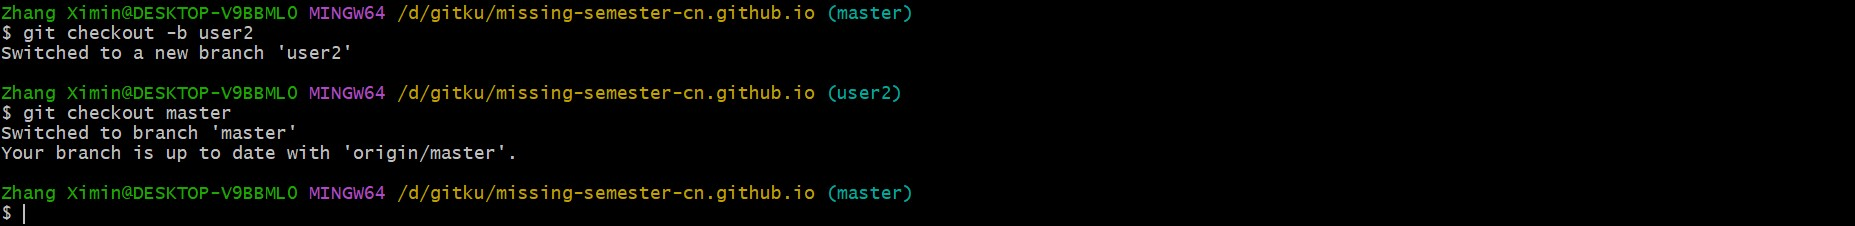
\includegraphics[width=1\textwidth]{024.jpg}
	\end{figure}
	
	\paragraph{(10)	git merge <revision>:}	
 	合并到当前分支。
	
	\begin{figure}[H]
		\centering
		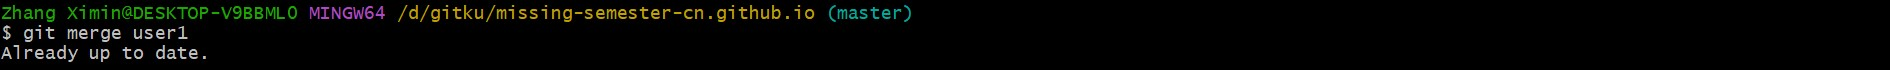
\includegraphics[width=1\textwidth]{025.jpg}
	\end{figure}
	
	\paragraph{(11)git rebase:}	
	将一系列补丁变基(rebase)为新的基线。
	
	使用 Rebase 方式将分支 B 并入分支 A 时,在 B 分支上的每一次 commit 都会单独添加到 A 分支,而不再像 Merge 方式那样创建一个合并 commit 来合并两个分支的内容。
	
	\begin{figure}[H]
		\centering
		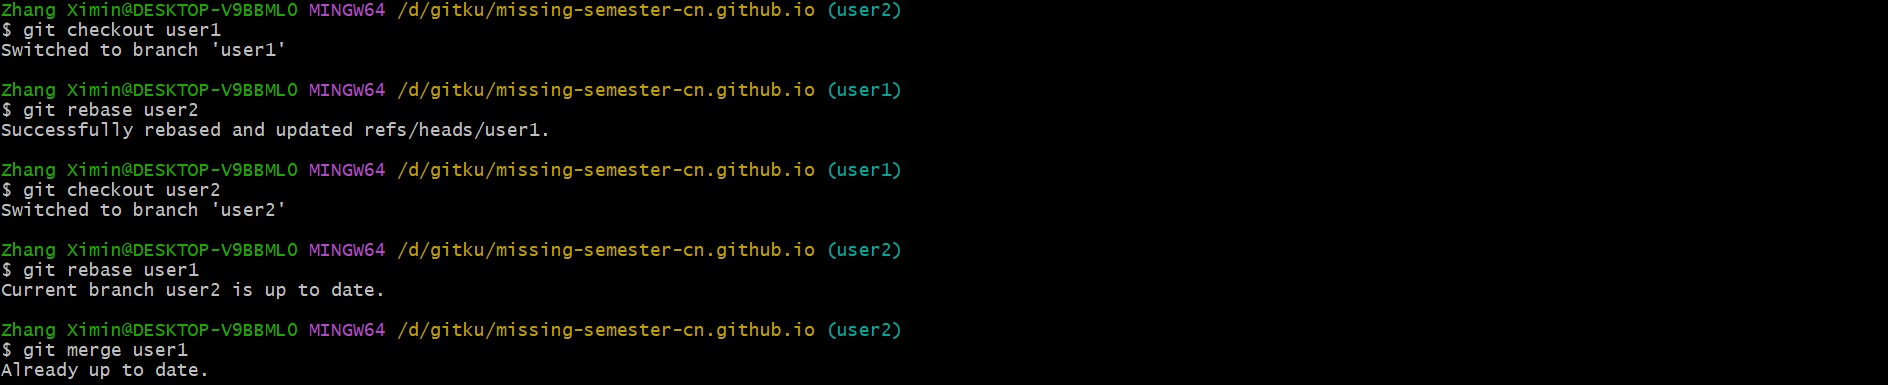
\includegraphics[width=1\textwidth]{027.jpg}
	\end{figure}
	
	\paragraph{(12)git remote:}	
	列出远端。
	
	git remote show <name>:查看某个远程仓库的详细信息。
	
	\begin{figure}[H]
		\centering
		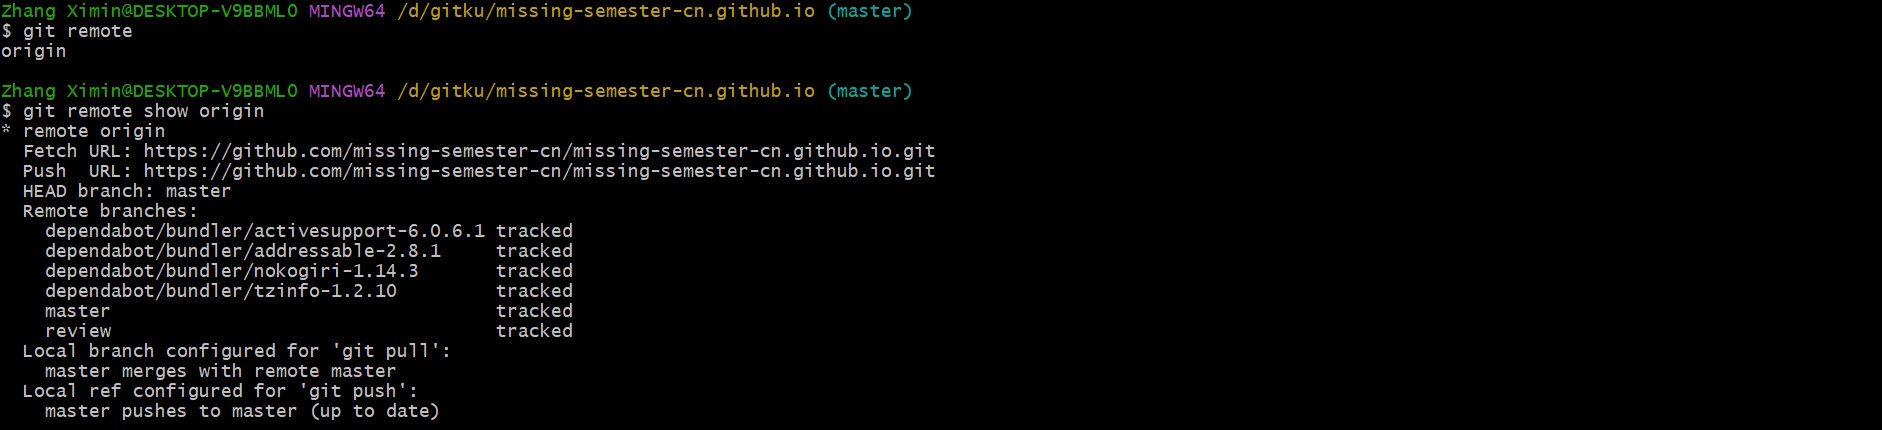
\includegraphics[width=1\textwidth]{028.jpg}
	\end{figure}
	
	\paragraph{(13)git fetch:}	
	从远端获取对象/索引。
	
	\begin{figure}[H]
		\centering
		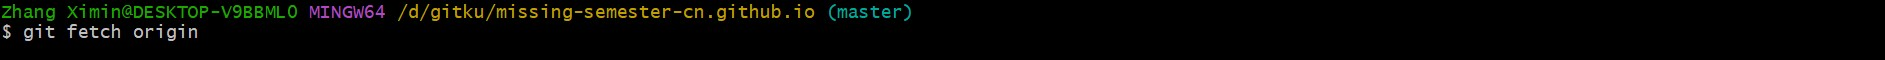
\includegraphics[width=1\textwidth]{029.jpg}
	\end{figure}
	
	\paragraph{(14)git clone:}	
	从远端下载仓库。
	
	\begin{figure}[H]
		\centering
		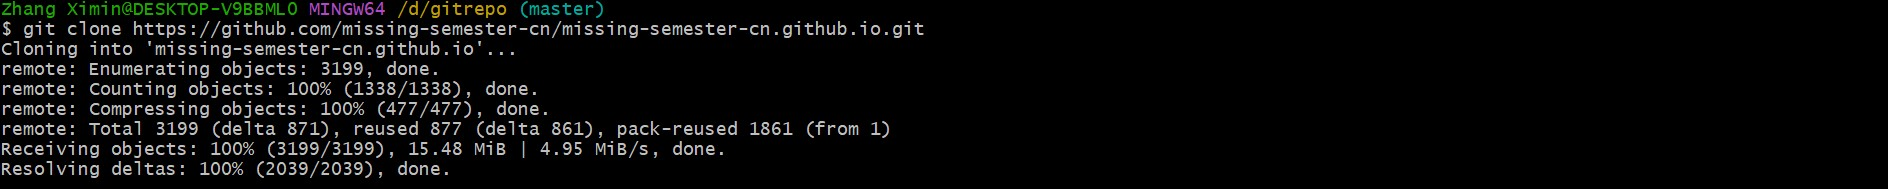
\includegraphics[width=1\textwidth]{030.jpg}
	\end{figure}
	
	\paragraph{(15)git remote add <name> <url>:}	
	添加一个远端。
	
	\begin{figure}[H]
		\centering
		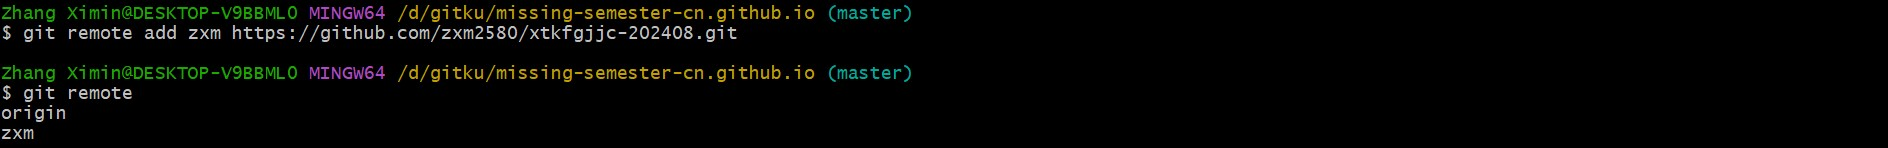
\includegraphics[width=1\textwidth]{031.jpg}
	\end{figure}
	
	\paragraph{(16)git remote rename <oldname> <newname>:}
	可以将名字为 oldname 的远程仓库改名为 newname。	
	
	\begin{figure}[H]
		\centering
		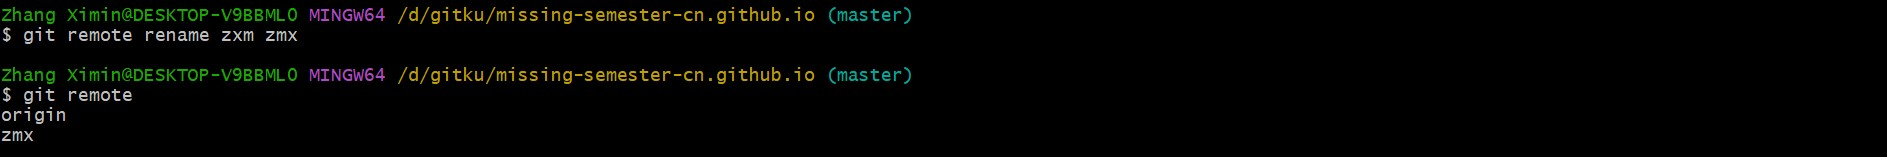
\includegraphics[width=1\textwidth]{032.jpg}
	\end{figure}
	
	\paragraph{(17)git remote get-url <name>:}
	查看名字为 name 的远程仓库的链接。	
	
	\begin{figure}[H]
		\centering
		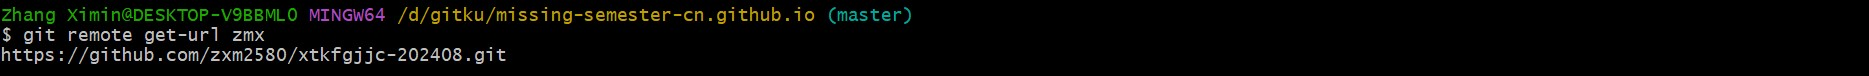
\includegraphics[width=1\textwidth]{033.jpg}
	\end{figure}
	
	\paragraph{(18)git remote set-url <name> <newurl>:}
	将名字为 name 的远程仓库的链接更改为 newurl。
	
	\begin{figure}[H]
		\centering
		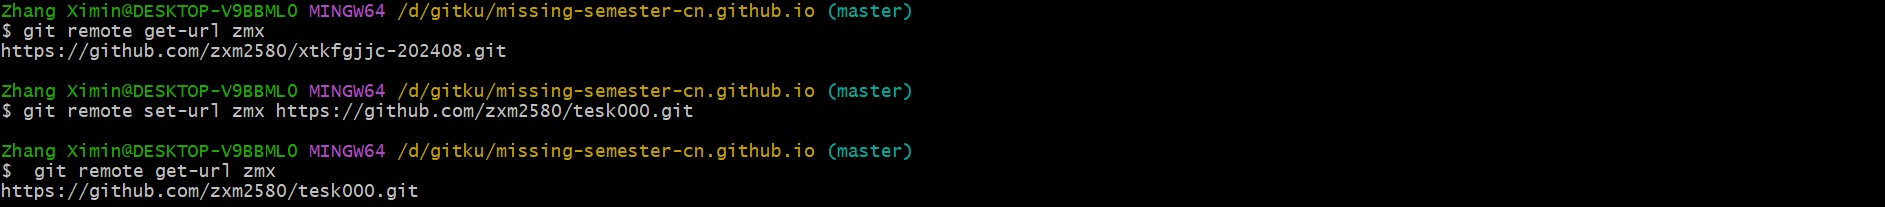
\includegraphics[width=1\textwidth]{034.jpg}
	\end{figure}
	
	\paragraph{(19)git remote rm <name>:}
	删除名字为 name 的远程仓库。
	
	\begin{figure}[H]
		\centering
		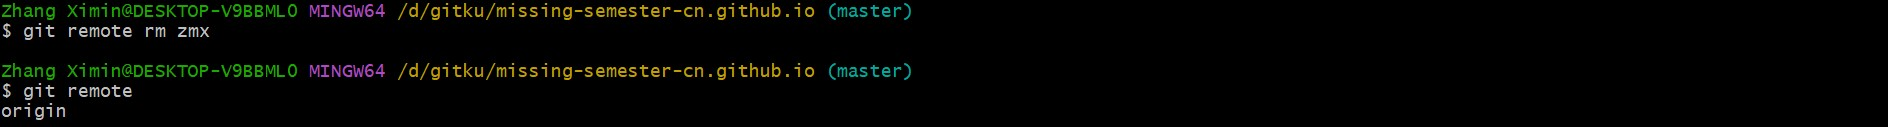
\includegraphics[width=1\textwidth]{035.jpg}
	\end{figure}
	
	\paragraph{(20)git pull <remote-name> <branch>:}
	获取 <remote-name> 的更改,然后将这些更改合并到分支。
	
	在默认情况下,git pull 相当于 git fetch 后 git merge。
	
	\begin{figure}[H]
		\centering
		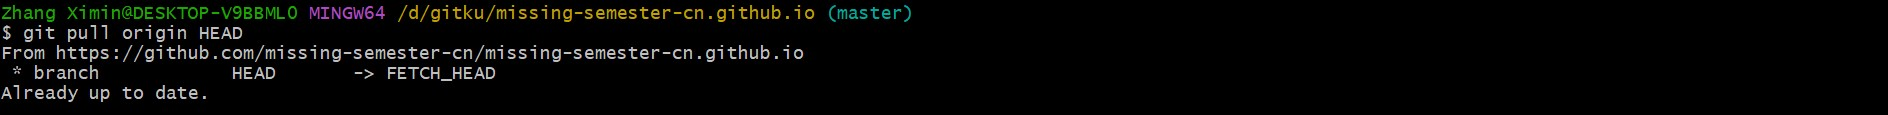
\includegraphics[width=1\textwidth]{036.jpg}
	\end{figure}
	
	\section{问题及解决方案}
	
	\paragraph{(1)}
	问题:使用git克隆库时报错:git schannel: crypt e no revocation checkout。
	
	解决方案:查找问题发现该报错通常是因为 Git 无法连接到证书撤销列表(CRL)服务器或者在本地配置中禁用了撤销检查。尝试配置 Git 以允许对证书撤销状态进行跳过。运行命令:git config--global http.sslVerify false 之后再git clone即可。后续发现本人这里的报错原因其实是本地网络无法连接到github网站,开启网络加速后再git clone即不报错。
	
	\begin{figure}[h]
		\centering
		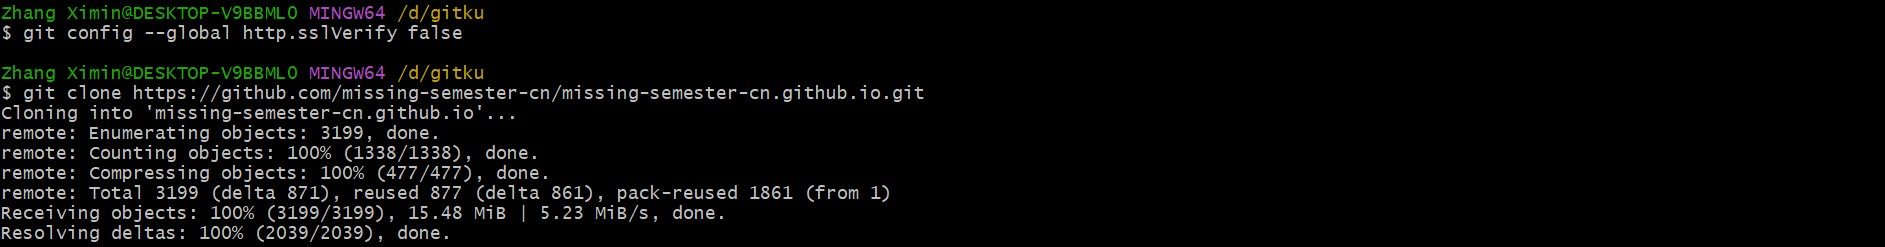
\includegraphics[width=1\textwidth]{99.jpg}
	\end{figure}
	
	\paragraph{(2)}
	问题:安装Latex时报错,如下:
	
	\begin{figure}[H]
		\centering
		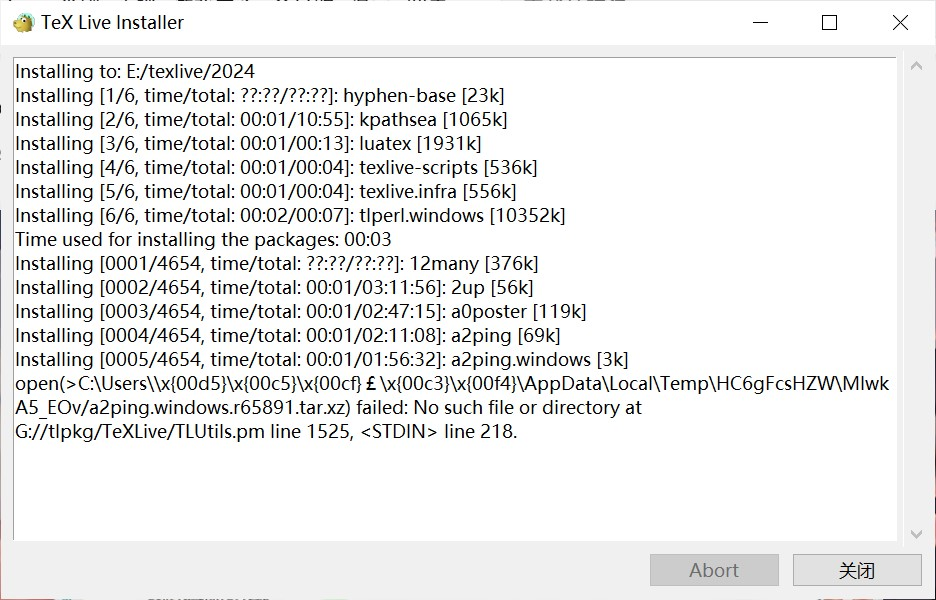
\includegraphics[width=1\textwidth]{102.jpg}
	\end{figure}
	
	解决方案:用户名是中文导致安装程序找不到相关文件。修改环境变量使其绕过中文路径即可。
	
	\begin{figure}[H]
		\centering
		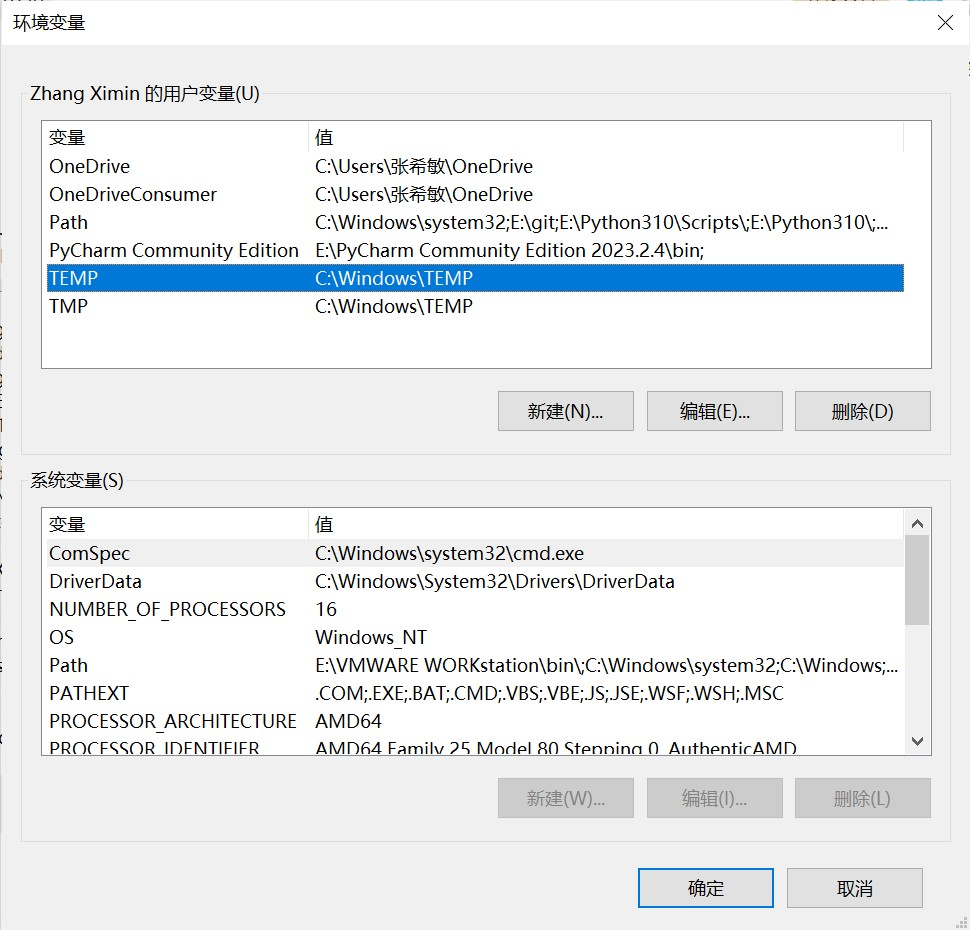
\includegraphics[width=1\textwidth]{103.jpg}
		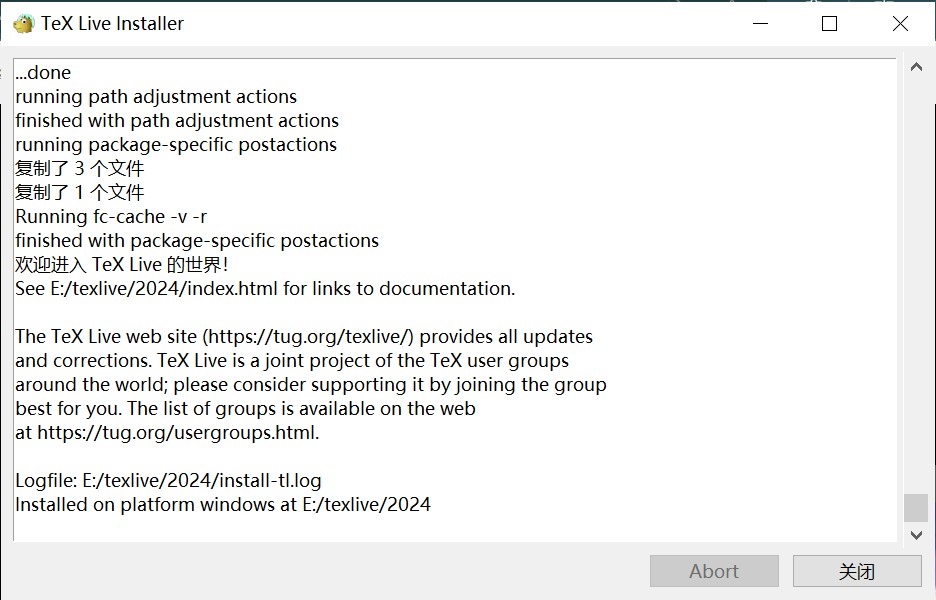
\includegraphics[width=1\textwidth]{104.jpg}
	\end{figure}
	
	\paragraph{(3)}
	问题:使用Latex插入图片时报错,如下:
	
	\begin{figure}[H]
		\centering
		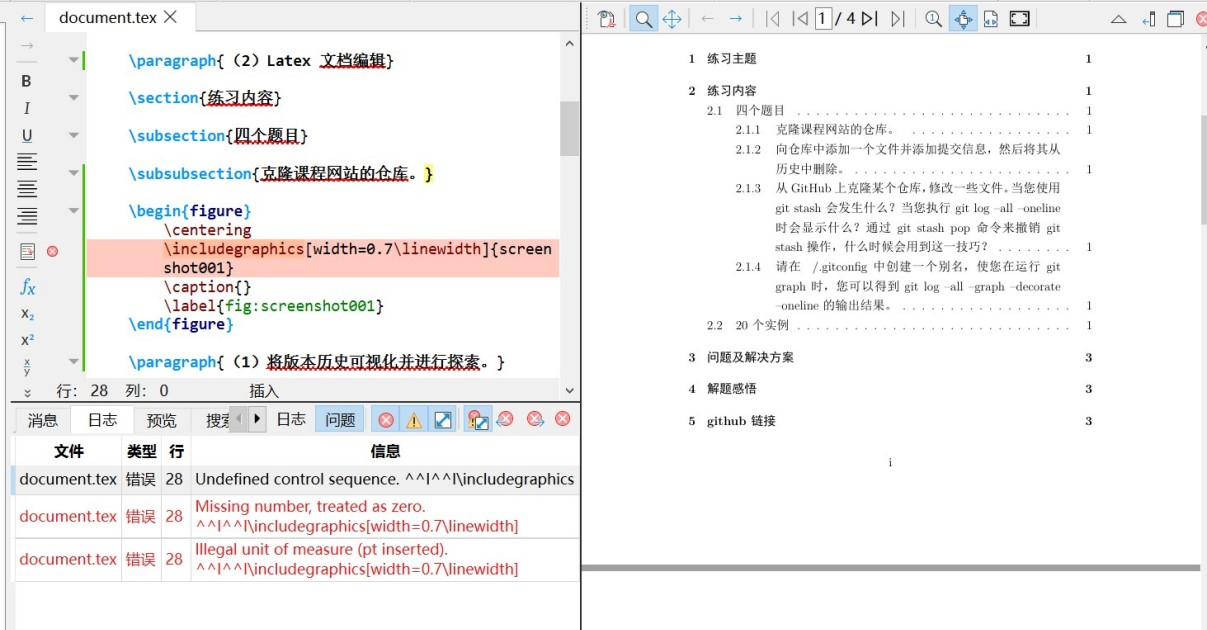
\includegraphics[width=1\textwidth]{100.jpg}
	\end{figure}
	
	解决方案:发现是忘记在导言区添加宏包了,添加后问题解决。
	
	\begin{figure}[H]
		\centering
		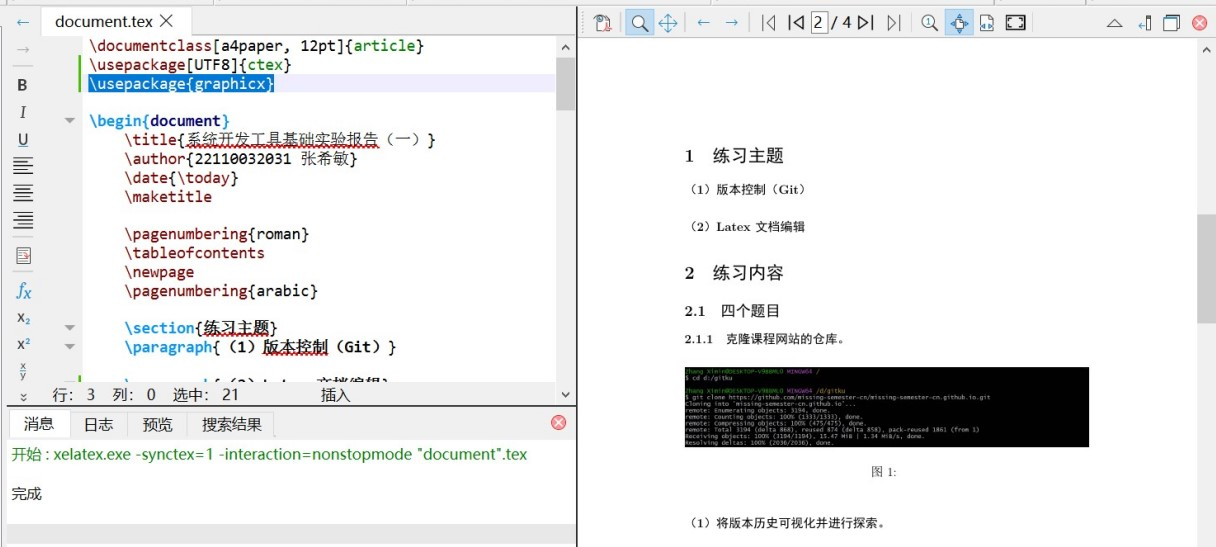
\includegraphics[width=1\textwidth]{101.jpg}
	\end{figure}
	
	\section{解题感悟}
	
	本实验中,我练习了关于Git版本控制和Latex文档编辑的内容,掌握了Git和Latex的基本操作。尤其在Git版本控制方面,我练习了克隆仓库、探索版本间的关系、添加并提交文件到仓库、切换不同分支、远端操作等方面的内容,受益匪浅。在Latex使用过程中我遇到许多问题,经过网络查询也得以解决,锻炼了我上手新工具和解决问题的能力。
	
	另外,我也体会到了Git和Latex在项目开发中的重要性。Git作为版本控制工具,能够帮助我们高效地管理代码和文档,大大提高我们的工作效率。而Latex则以其强大的排版功能和灵活的宏包系统,成为我们撰写技术文档的得力助手。
	
	\section{github链接}
	\underline{}	
	
\end{document}